%%%%%%%%%%%%%%%%%%%%%%%%%%%%%%%%%%%%%%%%%
% Proceedings of the National Academy of Sciences (PNAS)
% LaTeX Template
% Version 1.0 (19/5/13)
%
% This template has been downloaded from:
% http://www.LaTeXTemplates.com
%
% Original author:
% The PNAStwo class was created and is owned by PNAS:
% http://www.pnas.org/site/authors/LaTex.xhtml
% This template has been modified from the blank PNAS template to include
% examples of how to insert content and drastically change commenting. The
% structural integrity is maintained as in the original blank template.
%
% Original header:
%% PNAStmpl.tex
%% Template file to use for PNAS articles prepared in LaTeX
%% Version: Apr 14, 2008
%
%%%%%%%%%%%%%%%%%%%%%%%%%%%%%%%%%%%%%%%%%

%----------------------------------------------------------------------------------------
%	PACKAGES AND OTHER DOCUMENT CONFIGURATIONS
%----------------------------------------------------------------------------------------

%------------------------------------------------
% BASIC CLASS FILE
%------------------------------------------------

%% PNAStwo for two column articles is called by default.
%% Uncomment PNASone for single column articles. One column class
%% and style files are available upon request from pnas@nas.edu.

\documentclass[a4paper]{article}
%\documentclass{pnastwo}

%------------------------------------------------
% POSITION OF TEXT
%------------------------------------------------

%% Changing position of text on physical page:
%% Since not all printers position
%% the printed page in the same place on the physical page,
%% you can change the position yourself here, if you need to:

% \advance\voffset -.5in % Minus dimension will raise the printed page on the 
                         %  physical page; positive dimension will lower it.

%% You may set the dimension to the size that you need.

%------------------------------------------------
% GRAPHICS STYLE FILE
%------------------------------------------------

%% Requires graphics style file (graphicx.sty), used for inserting
%% .eps/image files into LaTeX articles.
%% Note that inclusion of .eps files is for your reference only;
%% when submitting to PNAS please submit figures separately.

%% Type into the square brackets the name of the driver program 
%% that you are using. If you don't know, try dvips, which is the
%% most common PC driver, or textures for the Mac. These are the options:

% [dvips], [xdvi], [dvipdf], [dvipdfm], [dvipdfmx], [pdftex], [dvipsone],
% [dviwindo], [emtex], [dviwin], [pctexps], [pctexwin], [pctexhp], [pctex32],
% [truetex], [tcidvi], [vtex], [oztex], [textures], [xetex]

\usepackage{graphicx}
\usepackage{algorithmic}
\usepackage{algorithm2e}


%------------------------------------------------
% ADDITIONAL OPTIONAL STYLE FILES
%------------------------------------------------

%% The AMS math files are commonly used to gain access to useful features
%% like extended math fonts and math commands.

\usepackage{amssymb,amsfonts,amsmath}

%------------------------------------------------
% OPTIONAL MACRO FILES
%------------------------------------------------

%% Insert self-defined macros here.
%% \newcommand definitions are recommended; \def definitions are supported

%\newcommand{\mfrac}[2]{\frac{\displaystyle #1}{\displaystyle #2}}
%\def\s{\sigma}


\begin{document}

%----------------------------------------------------------------------------------------
%	TITLE AND AUTHORS
%----------------------------------------------------------------------------------------

\title{Report on Machine Learning Lab, Ex 2} % For titles, only capitalize the first letter


\author{Mostafa Mohamed, Omar Kassem}%\affil{1}{Alberts-Ludwig Universt\"at Freiburg}}
%James Smith\affil{2}{University of Oregon}
%\and
%Jane Smith\affil{1}{}}

%\contributor{Submitted to Proceedings of the National Academy of Sciences of the United States of America}

%----------------------------------------------------------------------------------------

\maketitle % The \maketitle command is necessary to build the title page

%\begin{article}

%----------------------------------------------------------------------------------------
%	ABSTRACT, KEYWORDS AND ABBREVIATIONS
%----------------------------------------------------------------------------------------

%\begin{abstract}
%Abstract
%\end{abstract}

\section{Introduction}
This is a report about the deep learning lab, exercise 2. The general task of this assignment was to use Tensorflow to implement a convolutional neural network to train it on labelling images. As well as, trying different architectures for the network and different sizes.

\section{Data}
The training data set that consists of nearly 28,000 images, that mostly contain a lot of images about some objects; for each object we have similar images but with variants in some features, like brightness, color, the viewing angle. Then we used a validation data set of nearly 5,400 images and a testing data set of nearly 6,100 images.

\section{Tensorflow}
Tensorflow is a machine learning opensource software library (developed by Google) for running large computations on data flow graphs. It's architecture allows parallel computation on different GPUs. It also provides a variety of control statements over data flow graphs.

\section{Architecture}
We used a convolutional neural network of 2 layers in some tests and 3 layers in some other tests, we tried a variety of number of neurons in layers. This 3rd layer has shown an improvement on some of the results. All the datasets were batched, and in some of the runs we tried to shuffle some of the training data sets before batching in order to avoid overfitting.

\section{Results}
We tried training the network using 2 layers sometimes and 3 layers some other times, we present here a plot of the results for each of them when we run on 3 channels(RGB) and 4 channels(RGBD).

%----------------------------------------------------------------------------------------
%	FIGURES AND TABLES
%----------------------------------------------------------------------------------------

%% Adding Figure and Table References
%% Be sure to add figures and tables after \end{article}
%% and before \end{document}

%% For figures, put the caption below the illustration.
%%
%% \begin{figure}
%% \caption{Almost Sharp Front}\label{afoto}
%% \end{figure}

\begin{figure}[h]
\centerline{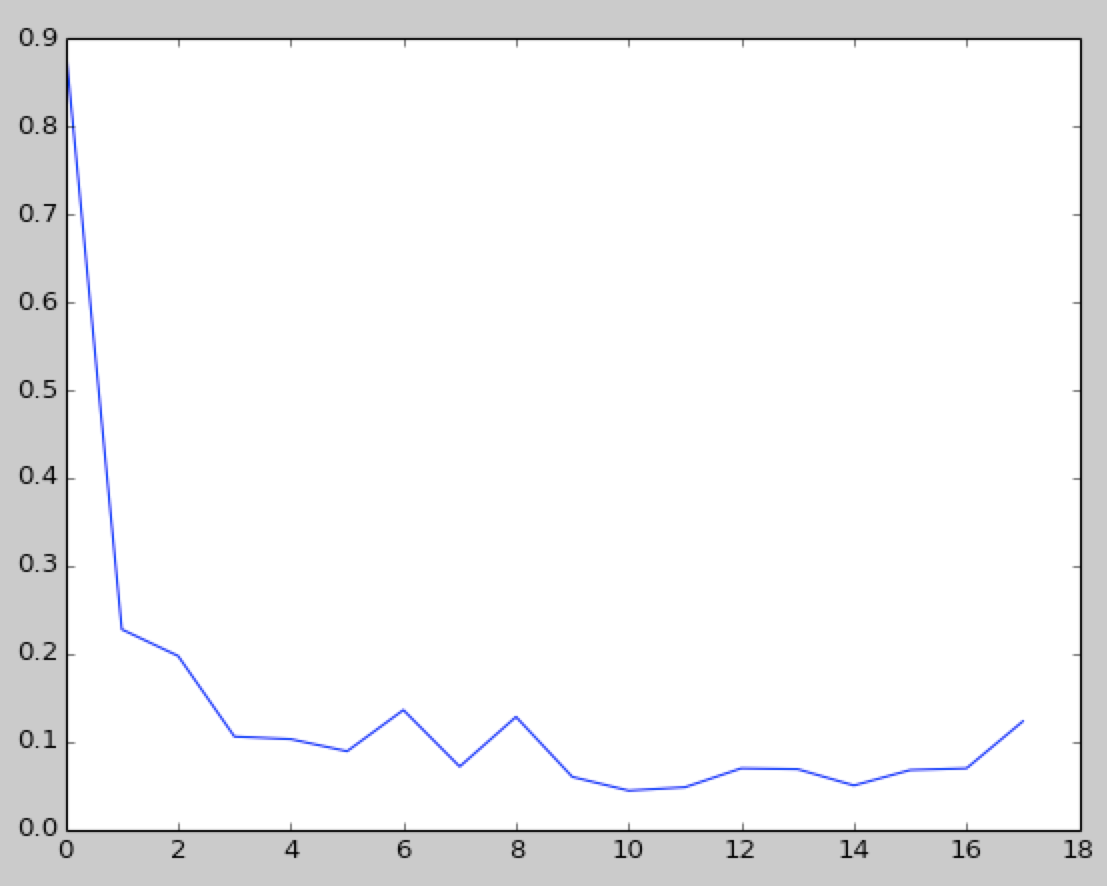
\includegraphics[width=0.4\linewidth]{2L3C.png}}
\caption{2 Layers, 3 Channels, Accuracy: 89\%}\label{placeholder}
\end{figure}

\begin{figure}[h]
\centerline{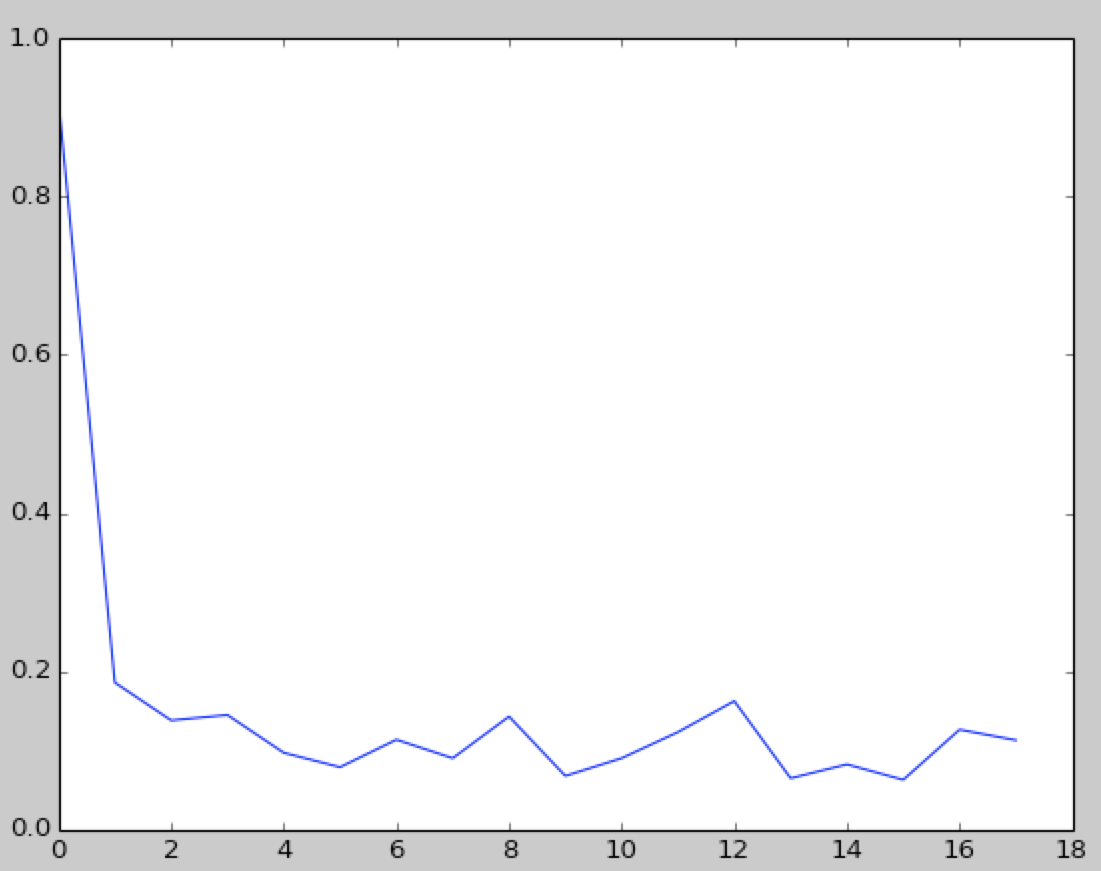
\includegraphics[width=0.4\linewidth]{2L4C.png}}
\caption{2 Layers, 4 Channels, Accuracy: 91\%}\label{placeholder}
\end{figure}

\begin{figure}[h]
\centerline{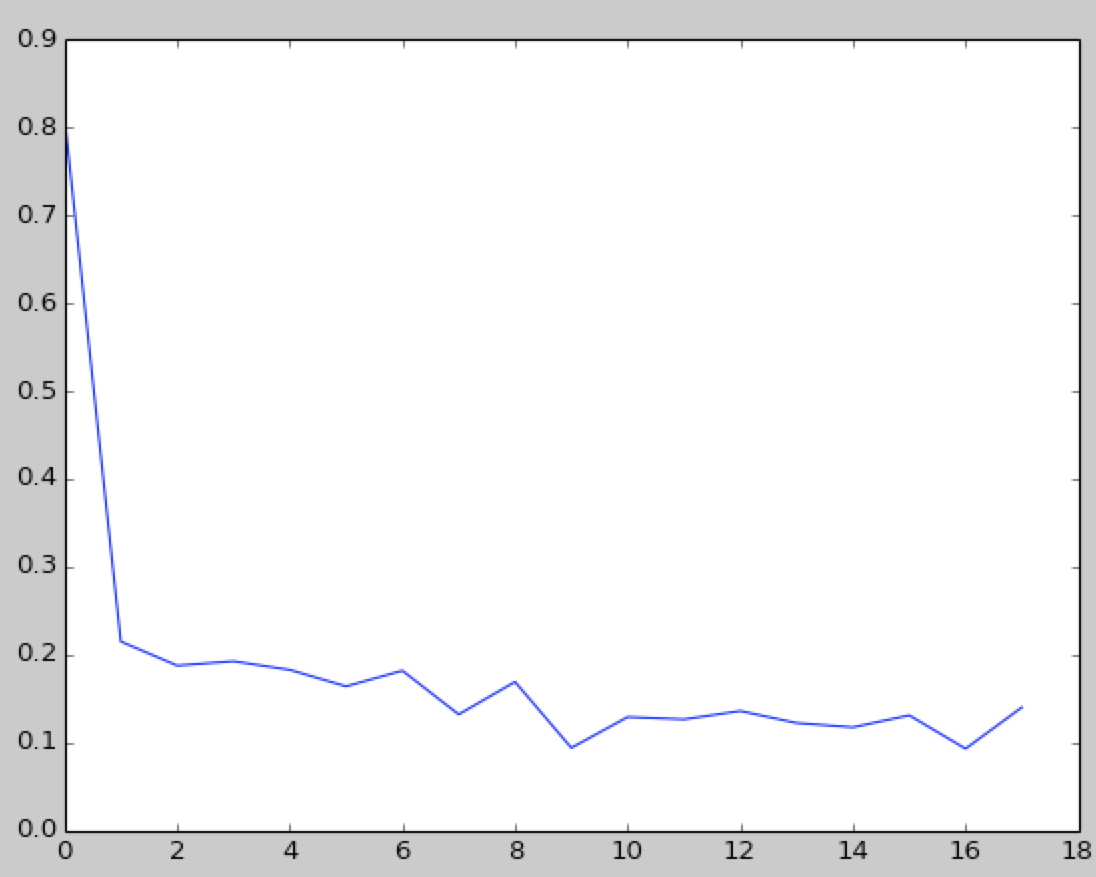
\includegraphics[width=0.4\linewidth]{3L3C.png}}
\caption{3 Layers, 3 Channels, Accuracy: 92\%}\label{placeholder}
\end{figure}

\begin{figure}[h]
\centerline{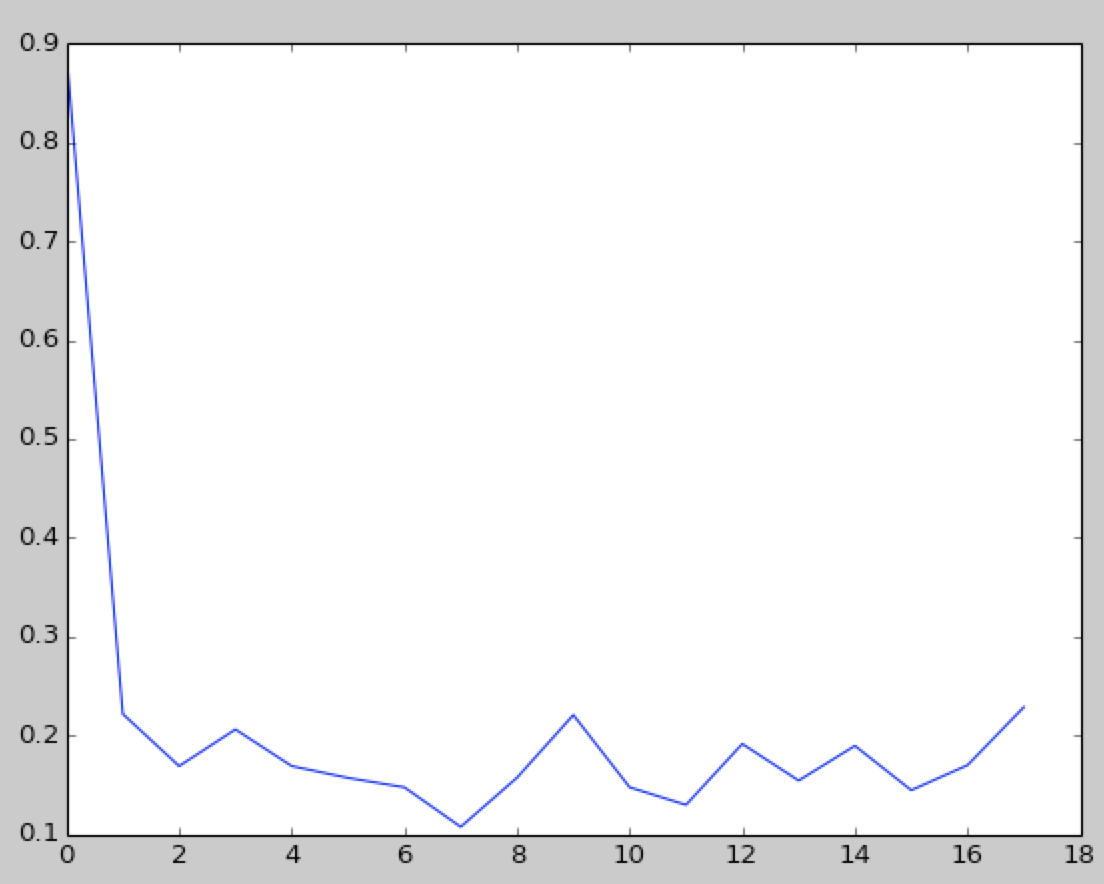
\includegraphics[width=0.4\linewidth]{3L4C.png}}
\caption{3 Layers, 4 Channels, 87\%}\label{placeholder}
\end{figure}

%% For Tables, put caption above table
%%
%% Table caption should start with a capital letter, continue with lower case
%% and not have a period at the end
%% Using @{\vrule height ?? depth ?? width0pt} in the tabular preamble will
%% keep that much space between every line in the table.

%% \begin{table}
%% \caption{Repeat length of longer allele by age of onset class}
%% \begin{tabular}{@{\vrule height 10.5pt depth4pt  width0pt}lrcccc}
%% table text
%% \end{tabular}
%% \end{table}

%% For two column figures and tables, use the following:

%% \begin{figure*}
%% \caption{Almost Sharp Front}\label{afoto}
%% \end{figure*}

%% \begin{table*}
%% \caption{Repeat length of longer allele by age of onset class}
%% \begin{tabular}{ccc}
%% table text
%% \end{tabular}
%% \end{table*}

%----------------------------------------------------------------------------------------

\end{document}
